\chapter{Einige wichtige Hinweise zum Arbeiten mit \LaTeX\ }
\label{sec:latexumg}

Throughout this work the following notation is employed: $W$ denotes
the world frame, $C_1$ or $C_2$ denotes a camera frame.  $T_{AB}$ is
the transformation from frame $A$ to frame $B$, measured in frame $A$.

$\vec{X}$ the position of the event with respect to world or camera
frame, $\vec{x}$ the calibrated coordinates of the event.

\section{From Events to Frame}
\label{sec:event_warp}
We group a set of events $\mathscr{E}\doteq \{e_k\}_{k=1}^N$ into a
temporal window, optimize the motion and scene parameters within this
window, then shift the window to the next set of events and repeat
this process. The temporal window size is defined by the event numbers
$N$, which should be chosen small enough so that a constant velocity
model could be applied within this window. We choose event numbers
against a fixed time interval to define the window size, because this
corresponds to the data-driven nature of an event-based camera: the
more rapid the apparent motion of the scene is, the larger the event
rate will be. If the scene stops moving, no events will be generated,
the pose will also not be further updated.

An event frame is thus formed by summing up events within this
window. If we simply sum along the time axis, the intensity at each
pixel will be the sum of the polarities of all the events that are
triggered at this pixel location within the window
\begin{equation}
  \label{eq:intensity}
  \mathcal{I}(\vec{x}) = \sum_1^N\pm_k(\vec{x}-\vec{x}_k),
\end{equation}
with $\pm_k$ and $\vec{x}_k$ denoting the polarity and pixel
coordinates of the $k$th event, respectively. After warping the events
with $\vec{x}'_k=\mat{W}(\vec{x}_k,t;\theta)$, we substitute
$\vec{x}_k$ in the above equation to $\vec{x}'_k$.

\subsection{Measuring the Sharpness of an Image}
\label{sec:contrast}
\begin{equation}
  \label{eq:variance}
  \mathrm{Var}\doteq\frac{1}{\mid\Omega\mid}\int_{\Omega}\left(\mathcal{I}\left(\vec{x}\right)-\mu\left(\mathcal{I}\left(\vec{x}\right)\right)\right)^2d\vec{x}
\end{equation}


\subsection{Planar Homography}

\label{sec:planar_homo}
The warp function $\vec{x}'=\mat{W}(\vec{x},t;\theta)$ does
not only depend on the motion parameters, but also the scene
parameters, which is the unknown depth.  In the case of a planar scene
the problems simplifies, since a plane $\mathbf{P}$ can be
parameterized by two sets of parameters: $\vec{n}\in\mathbb{S}^2$ the
unit surface normal of $\mathbf{P}$ with respect to the current camera
frame, and $d$ the distance from the camera center to
$\mathbf{P}$. The warp function then becomes
\begin{align}
  \vec{X}'=&\mat{R}\vec{X}+\vec{T}\\
  \vec{X}=&\mat{R}^\top\left(\vec{X}'-\vec{T}\right)\\
  \vec{X}=&\mat{R}^\top\left(\mat{I}+\vec{T}\vec{n}^\top/d\right)\vec{X}',  \label{eq:planar_homo_0}
\end{align}
thus
$\vec{x}'\sim\left(\mat{R}^\top\left(\mat{I}+\vec{T}\vec{n}^\top/d\right)\right)^{-1}\vec{x}$.
Here $(\mat{R}, \vec{T})\in SE(3)$ denotes the relative pose between
two cameras at which the current event being warped and the first
event within the window happened. Under a constant velocity model with
linear velocity $\vec{v}\in\mathbb{R}^3$ and angular velocity
$\bm{\omega}\in\mathbb{R}^3$, the translation is given by
\begin{equation}
  \label{eq:translation}
  \vec{T}(t)=\vec{v}t,
\end{equation}
the rotation matrix is given by the \textit{exponential map} exp:
$\mathfrak{so}(3)\rightarrow SO(3)$:
\begin{equation}
  \label{eq:rotation}
  \mat{R}(t)=\mathrm{exp}(\bm{\omega}^\wedge t),
\end{equation}
where $^\wedge$ is the \textit{hat} operator
\begin{equation}
  \label{eq:hat}
  \bm{\omega}^\wedge=
  \begin{bmatrix}
    \omega_1\\\omega_2\\\omega_3
  \end{bmatrix}
  =
  \begin{bmatrix}
    0&-\omega_3&\omega_2\\
    \omega_3&0&-\omega_1\\
    -\omega_2&\omega_1&0
  \end{bmatrix}
  \in\mathfrak{so}(3),
\end{equation}

\section{From Frames to Map}
\label{sec:frame2map}
The contrast maximization procedure in the above section optimizes the
relative pose between successive frames. We show in this section that
the same idea can be applied to perform global pose tracking in planar
scenes. We first explain how the map is defined, and how to track a
known map, then we shown how this map is built by selecting a set of
keyframes.

\subsection{Map}
\label{sec:map}
A map is a plane with normal direction $\vec{n}_w$ and distance $d_w$
to the origin; the texture of a map represents all the edges on the
plane. \Cref{fig:map} shows the an example of such
map. \Cref{fig:map}(a) also shows the set of keyframes used to
construct the map. We will talk more about keyframes in
\cref{sec:keyframe2map}. The global coordinate is chosen as the camera
coordinate of the first frame.

\begin{figure}
  \begin{minipage}[t]{0.48\textwidth}
    \centering 
\includegraphics[width =
    \textwidth]{images/map_805.jpg}
    % \label{subfig:texture}
    (a) The texture of a map
  \end{minipage}
  \hfill
  \begin{minipage}[t]{0.48\textwidth}
    \centering 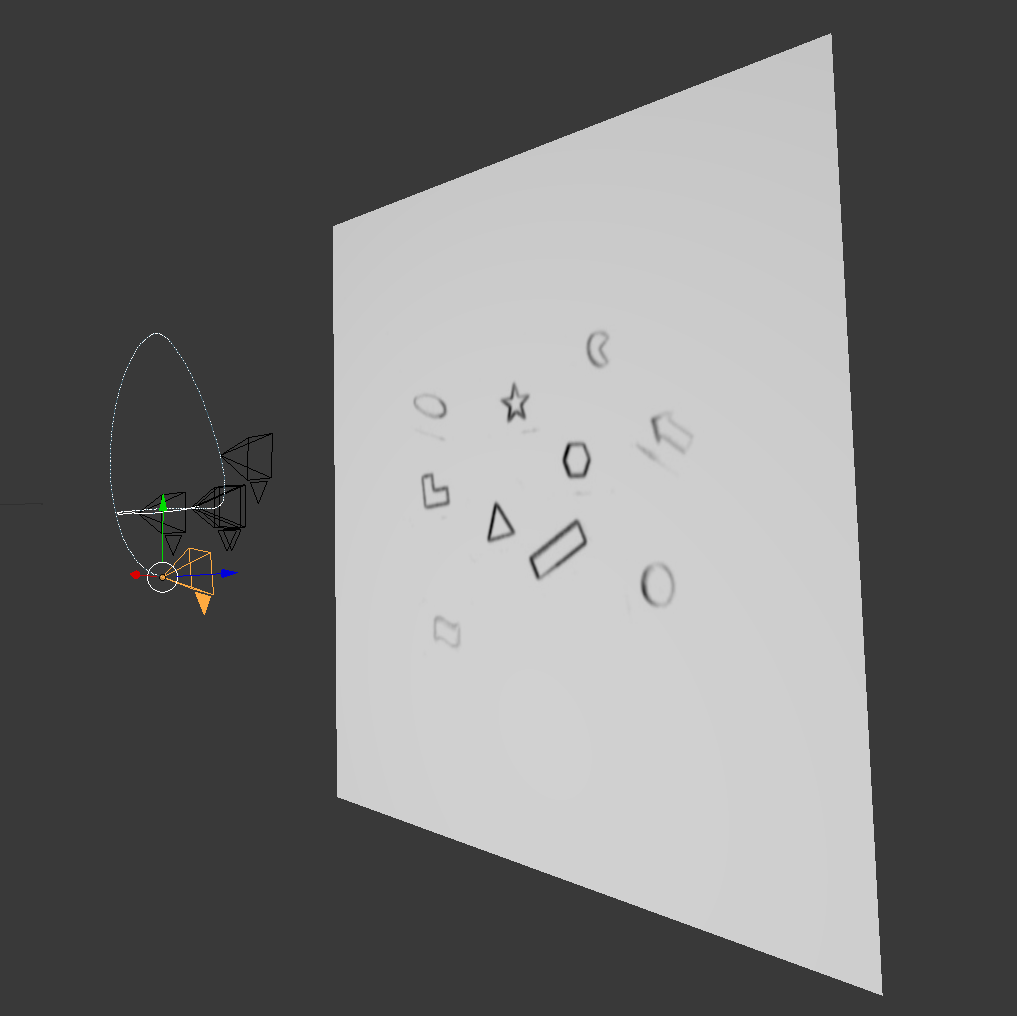
\includegraphics[width = \textwidth]{images/4.png}
    % \label{subfig:map}
    (b) A map in the global frame
  \end{minipage}
  \caption{Map}
  \label{fig:map}
\end{figure}




\subsection{Tracking}
\label{sec:tracking}
Suppose a map is present, then the normal direction $\vec{n}_w$ of the
plane and the distance $d_w$ to the origin are known. Also the pose of
the current frame $(\mat{R}_{wc}, \vec{T}_{wc})\in SE(3)$ is
determined by the motion estimation from the last frame (a quick note
to the terminology we are using: whenever we say the \textit{pose} of
a frame, we always refer to the camera \textit{pose} at which the
first event within the frame happens). The parameters left to be
estimated for each frame is
$\{\bm{\omega},\vec{v}\}\in\mathbb{R}^6$. By substituting $\vec{n}$
with $\vec{n}_c = \mat{R}_{cw}\vec{n}_w$, and $d$ with
$d_c = d_w+\vec{T}_{wc}\cdot\vec{n}_w$ in \cref{eq:planar_homo_0}, we
get the homography matrix within each frame as
\begin{equation}
  \label{eq:planar_homo_1}
  \mat{H}_1=\mat{R}^\top\left(\mat{I}+\vec{T}\vec{n}_c^\top/d_c\right)
\end{equation}
and $\vec{x}'_c\sim\mat{H}_1^{-1}x_c$.

A nonlinear optimizing problem naturally suffers from local
optima. Without a good initialization, the motion computed with the
method in \cref{sec:event_warp} could sometimes be a local optimum
delivering an image that appears sharp, despite being wrongly
estimated (see \cref{fig:local_optimum}). In order to make sure that
the estimated motion from the per frame contrast maximization also
conform to the global map. Thus we perform another optimization, where
we project the events of the current frame to the global map. The
parameter set is still $\{\bm{\omega},\vec{v}\}$, and we use the
output from last procedure as an initial guess.

The procedure described in the first paragraph of this section can be
understood as projecting the events on a \textit{blank
  canvas}. Similarly, in the projecting-to-map procedure we project
the events on the \textit{texture} of the map, and measure the
strength of the synthesized image with the same variance function as
in \cref{eq:variance}, thus finding the set of the parameters that
best align the events in the current frame to their correspondences in
the texture.

The projection from an event to the map is
$\vec{x}_w \sim \mat{R}_n\mat{H}_2^{-1}\mat{H}_1^{-1}\vec{x}_c$, with
$\mat{R}_n$ the transformation from the orientation of the global
frame to the orientation of the map, computed by
\begin{align}
  \label{eq:global2map}
  \mat{K}& =(\vec{n}_w\times \vec{z})^\wedge\\
  \mat{R}_n&=\mat{I} +\mat{K} + \mat{K}^2/ (1 +  \vec{n_w}\cdot\vec{z}),
\end{align}
where $\vec{z}=(0,0,-1)$ denotes the plane fronto-parallel to the
camera, and
\begin{equation}
  \label{eq:frame2global}
  \mat{H}_2 = \mat{R}_{cw}\left(\mat{I} + \vec{T}_{wc}\vec{n}^\top/d_w\right),
\end{equation}
the projection from the current frame to the global frame, with
$\mat{R}_{wc}, \mat{T}_{wc}$ being the pose of the current
frame. $\mat{H}_1$ is the planar homography for each frame as in
\cref{eq:planar_homo_1}. But the $\mat{R}$ and $\vec{T}$ might be
different since we are refining these parameters.
\begin{figure}
  \begin{minipage}[t]{0.48\textwidth}
    \centering 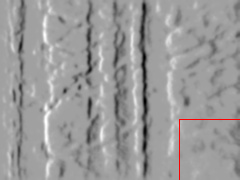
\includegraphics[width =
    \textwidth]{images/slider_estimation.png}
    \label{subfig:estimation}
    (a) Estimation
  \end{minipage}
  \hfill
  \begin{minipage}[t]{0.48\textwidth}
    \centering 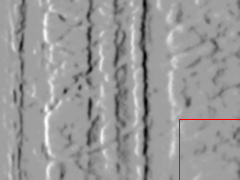
\includegraphics[width =
    \textwidth]{images/slider_groundtruth.png}
    \label{subfig:groundtruth}
    (b) Groundtruth
  \end{minipage}
  \hfill

  \begin{minipage}[t]{\textwidth}
    \centering 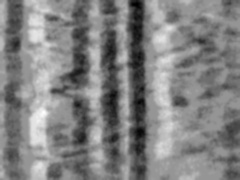
\includegraphics[width =
    0.48\textwidth]{images/slider_zero_motion.jpg}
    \label{subfig:estimation}
    \\(c) Without motion compensation
  \end{minipage}
  \hfill

  \caption{An example of local optima. This is the dataset
    \textit{slider\_hdr\_close} with a window size of 50000
    events. (a) shows the optimized image with \textit{linear
      velocity} $( 0.231, 0.109, 0.256)$, \textit{angular velocity}
    $(0.405, -0.130, -2.278)$ and \textit{plane normal}
    $(-0.579, 0.282, -0.765)$. (b) shows the result using groundtruth
    parameters with \textit{linear velocity} $(0.163, 0, 0)$,
    \textit{angular velocity} $(0, 0, 0)$ and \textit{plane normal}
    $(0, 0, -1)$. Both images appear mostly identical, though at the
    lower right corner, for example, one can still recognize the
    difference. Also both images look much sharper than the image
    without motion compensation in (c). It is worth mentioning that
    the contrast of the estimation is actually slightly larger than
    that of the groundtruth}
  \label{fig:local_optimum}
\end{figure}

\subsection{Mapping}
\label{sec:keyframe2map}


\subsection{note}
\label{sec:note}

tried initialize with multiple frames, didn't work very
well. similarly sliding window didn't work; too many events didn't
work

\chapter{Discussion}
\label{chap:discussion}



\section{Gliederungen}
\label{sec:gliederung}

Ein Text kann mit den Befehlen \texttt{\textbackslash chapter\{.\}},
\texttt{\textbackslash section\{.\}}, \texttt{\textbackslash
  subsection\{.\}} und \texttt{\textbackslash subsubsection\{.\}}
gegliedert werden.


\section{Referenzen und Verweise}
\label{sec:refverw}

Literaturreferenzen werden mit dem Befehl \texttt{\textbackslash
  citep\{.\}} und \texttt{\textbackslash citet\{.\}}
erzeugt. Beispiele: ein Buch
\citep{Raibert1986LeggedRobotsThatBalance}, ein Buch und ein Journal
Paper
\citep{Raibert1986LeggedRobotsThatBalance,Vukobratovic2004ZeroMomentPoint},
ein Konferenz Paper mit Erwähnung des Autors: \citet{Pratt1995SEA}.

Zur Erzeugung von Fussnoten wird der Befehl \texttt{\textbackslash
  footnote\{.\}} verwendet. Auch hier ein Beispiel\footnote{Bla bla.}.

Querverweise im Text werden mit \texttt{\textbackslash label\{.\}}
verankert und mit \texttt{\textbackslash cref\{.\}} erzeugt.  Beispiel
einer Referenz auf das zweite Kapitel: \cref{sec:latexumg}.


\section{Aufzählungen}\label{sec:aufz}

Folgendes Beispiel einer Aufzählung ohne Numerierung,
\begin{itemize}
\item Punkt 1
\item Punkt 2
\end{itemize}
wurde erzeugt mit:
\begin{verbatim}
\begin{itemize}
\item Punkt 1
\item Punkt 2
\end{itemize}
\end{verbatim}

Folgendes Beispiel einer Aufzählung mit Numerierung,
\begin{enumerate}
\item Punkt 1
\item Punkt 2
\end{enumerate}
wurde erzeugt mit:
\begin{verbatim}
\begin{enumerate}
\item Punkt 1
\item Punkt 2
\end{enumerate}
\end{verbatim}

Folgendes Beispiel einer Auflistung,
\begin{description}
\item[P1] Punkt 1
\item[P2] Punkt 2
\end{description}
wurde erzeugt mit:
\begin{verbatim}
\begin{description}
\item[P1] Punkt 1
\item[P2] Punkt 2
\end{description}
\end{verbatim}


\section{Erstellen einer Tabelle}\label{sec:tabellen}

Ein Beispiel einer Tabelle:
\begin{table}[h]
  \begin{center}
    \caption{Daten der Fahrzyklen ECE, EUDC, NEFZ.}\vspace{1ex}
    \label{tab:tabnefz}
    \begin{tabular}{ll|ccc}
      \hline
      Kennzahl & Einheit & ECE & EUDC & NEFZ \\ \hline \hline
      Dauer & s & 780 & 400 & 1180 \\
      Distanz & km & 4.052 & 6.955 & 11.007 \\
      Durchschnittsgeschwindigkeit & km/h & 18.7 &  62.6 & 33.6 \\
      Leerlaufanteil & \% & 36 & 10 & 27 \\
      \hline
    \end{tabular}
  \end{center}
\end{table}

Die Tabelle wurde erzeugt mit:
\begin{verbatim}
\begin{table}[h]
  \begin{center}
    \caption{Daten der Fahrzyklen ECE, EUDC, NEFZ.}\vspace{1ex}
    \label{tab:tabnefz}
    \begin{tabular}{ll|ccc}
      \hline
      Kennzahl & Einheit & ECE & EUDC & NEFZ \\ \hline \hline
      Dauer & s & 780 & 400 & 1180 \\
      Distanz & km & 4.052 & 6.955 & 11.007 \\
      Durchschnittsgeschwindigkeit & km/h & 18.7 &  62.6 & 33.6 \\
      Leerlaufanteil & \% & 36 & 10 & 27 \\
      \hline
    \end{tabular}
  \end{center}
\end{table}
\end{verbatim}


\section{Einbinden einer Grafik}\label{sec:epsgraph}

Das Einbinden von Graphiken kann wie folgt bewerkstelligt werden:
\begin{verbatim}
\begin{figure}
  \centering 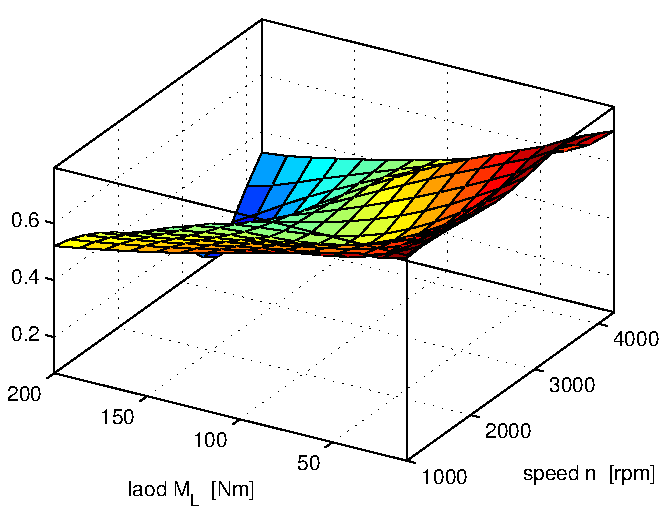
\includegraphics[width=0.75\textwidth]{images/k_surf.pdf}
  \caption{Ein Bild.}
  \label{fig:k_surf}
\end{figure}
\end{verbatim}

\begin{figure}
  \centering 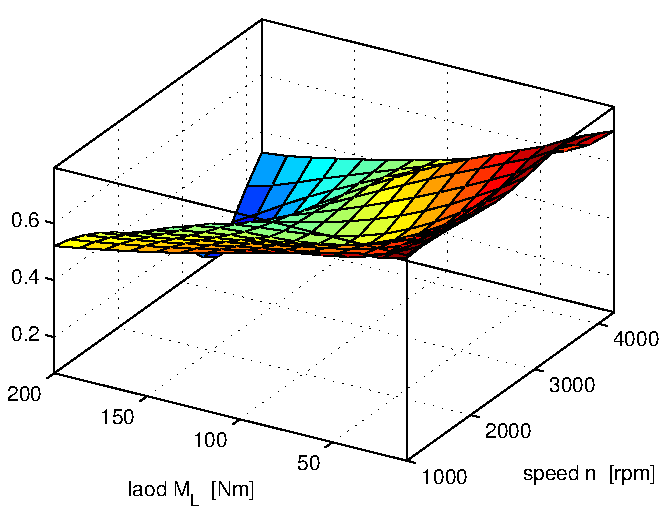
\includegraphics[width=0.75\textwidth]{images/k_surf.pdf}
  \caption{Ein Bild}
  \label{pics:k_surf}
\end{figure}

oder bei zwei Bildern nebeneinander mit:
\begin{verbatim}
\begin{figure}
  \begin{minipage}[t]{0.48\textwidth}
    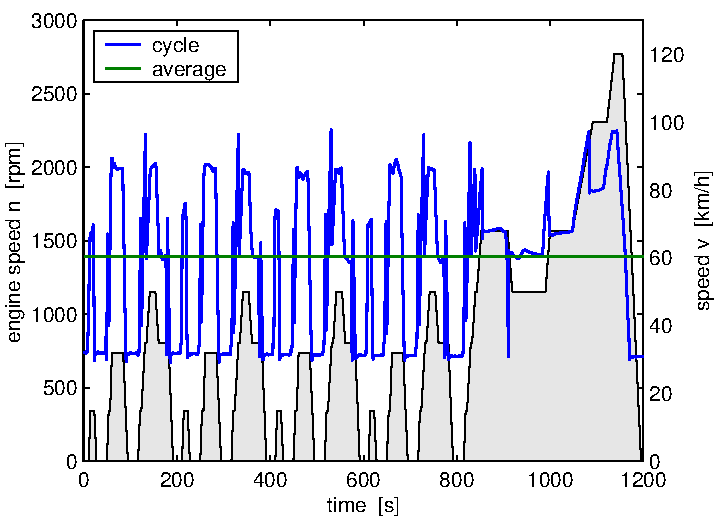
\includegraphics[width = \textwidth]{images/cycle_we.pdf}
  \end{minipage}
  \hfill
  \begin{minipage}[t]{0.48\textwidth}
    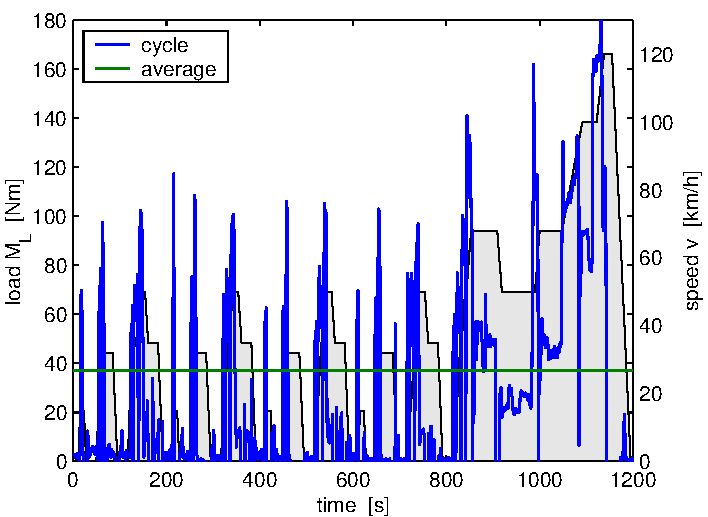
\includegraphics[width = \textwidth]{images/cycle_ml.pdf}
  \end{minipage}
  \caption{Zwei Bilder nebeneinander.}
  \label{pics:cycle}
\end{figure}
\end{verbatim}

\begin{figure}
  \begin{minipage}[t]{0.48\textwidth}
    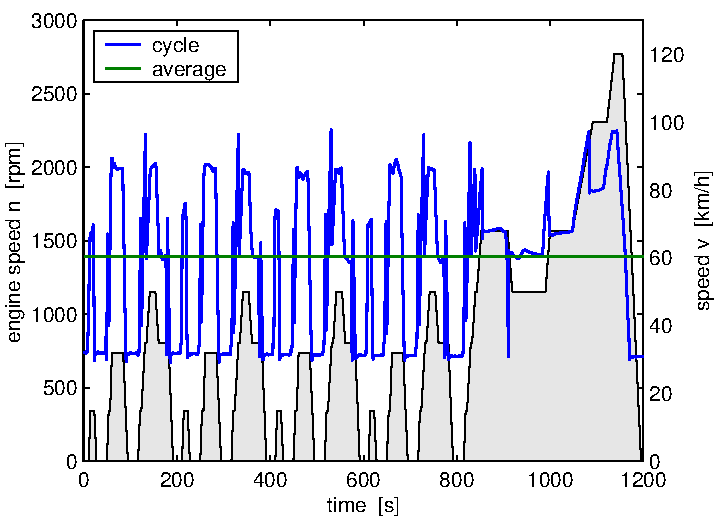
\includegraphics[width = \textwidth]{images/cycle_we.pdf}
  \end{minipage}
  \hfill
  \begin{minipage}[t]{0.48\textwidth}
    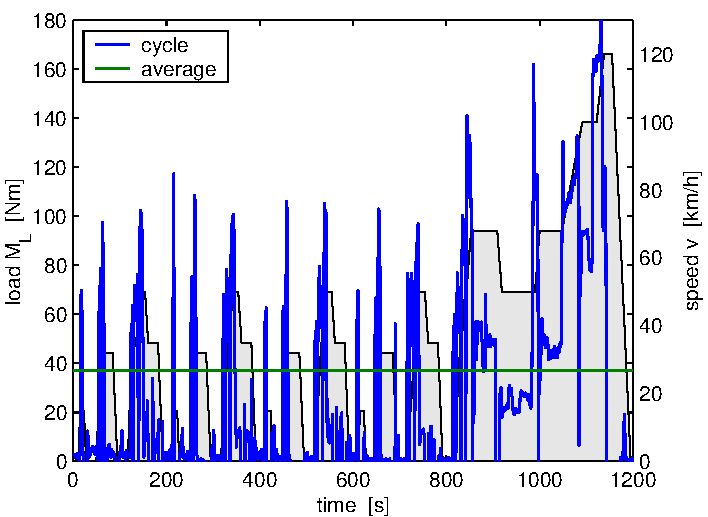
\includegraphics[width = \textwidth]{images/cycle_ml.pdf}
  \end{minipage}
  \caption{Zwei Bilder nebeneinander}
  \label{pics:cycle}
\end{figure}


\section{Mathematische Formeln}\label{sec:math}

Einfache mathematische Formeln werden mit der equation-Umgebung
erzeugt:
\begin{equation}
  p_{me0f}(T_e,\omega_e) \ = \ k_1(T_e) \cdot (k_2+k_3 S^2
  \omega_e^2) \cdot \Pi_{\mathrm{max}} \cdot \sqrt{\frac{k_4}{B}} \, .
  \label{eq:my_equation}
\end{equation}

Der Code dazu lautet:
\begin{verbatim}
\begin{equation}
  p_{me0f}(T_e,\omega_e) \ = \ k_1(T_e) \cdot (k_2+k_3 S^2
  \omega_e^2) \cdot \Pi_{max} \cdot \sqrt{\frac{k_4}{B}} \, .
\end{equation}
\end{verbatim}

Mathematische Ausdrücke im Text werden mit \$formel\$ erzeugt (z.B.:
$a^2+b^2=c^2$).

Vektoren und Matrizen werden mit den Befehlen \texttt{\textbackslash
  vec\{.\}} und \texttt{\textbackslash mat\{.\}} erzeugt
(z.B. $\vec{v}$, $\mat{M}$).


\section{Weitere nützliche Befehle}\label{sec:div}

Hervorhebungen im Text sehen so aus: \emph{hervorgehoben}. Erzeugt
werden sie mit dem \texttt{\textbackslash epmh\{.\}} Befehl.

Einheiten werden mit den Befehlen \texttt{\textbackslash unit[1]\{m\}}
(z.B.~\unit[1]{m}) und \texttt{\textbackslash unitfrac[1]\{m\}\{s\}}
(z.B.~\unitfrac[1]{m}{s}) gesetzt.
